\documentclass{llncs}

\usepackage[utf8]{inputenc}

\usepackage{amsmath}
\usepackage{amssymb}
\usepackage{booktabs} % needed for specialrule in tables
\usepackage{graphicx}
\usepackage{hyperref}
\usepackage{makecell} % needed for table headings and line breaks in cells
\usepackage{paralist}
\usepackage{footmisc}
\usepackage[parfill]{parskip} % don't indent text after newlines
\usepackage[most]{tcolorbox} % needed for todos in a different background color
\usepackage{wrapfig} % wrapping text around tables

% makecell table definitions
\renewcommand\theadalign{bc}
\renewcommand\theadfont{\bfseries}
\renewcommand\theadgape{\Gape[0.4em]}
\renewcommand\cellgape{\Gape[0.2em]}
\renewcommand{\cellalign}{l}

% custom commands
\newcommand{\crowdre}{Crowd RE} % Name of the data set
\newcommand{\blockcomment}[1]{}

\title{Topic Modeling on the Crowd RE Dataset using Unsupervised Machine Learning}
\author{Nicholas Alan Andrew Patrick Ford, Kim Julian Gülle}

\institute{
Technische Universität Berlin\\
\email{nicholas.ford@campus.tu-berlin.de, kim.j.guelle@campus.tu-berlin.de}\\ 
}

\begin{document}
\maketitle

\begin{abstract}
We aimed to automatically derive topics from a dataset of 2966 requirement sentences. The requirements were previously collected, tagged and categorized by crowd workers as part of the \crowdre{} project. We preprocessed the data in an NLP pipeline using state of the art NLP methods and applied topic modeling techniques to the results in order to cluster the data. This includes Latent Dirichclet Allocation, word embeddings using word2vec and the recently published Word Mover's Distance. We visiualized our findings in 2D scatter plots with the help of Principal Component Analysis and Stochastic Neighbor Embedding (t-SNE). All our programming work was done in Python and is strongly dependend on the nltk and gensim library.
The requirement sentences had 5 different domains already assigned to them (including a domain called \emph{Other}, which was neither of the other 4). Thus we expected to find 4 different clusters, with some noise between them, caused by the requirements of the \emph{Other} domain. Having followed several approaches for topic modeling we found out that the Word Mover's Distance is probably the most promising, still we were only able to find 3 reasonably distinct clusters. The final verification, whether this means the pre-assigned categories are wrong or the dataset is too small for an automated topic modeling (or a combination of both) is a manual process and may be part of future work.
\end{abstract}

%-- Main Content
\section{Introduction} % (fold)
\label{sec:introduction}
\blockcomment{
	The result of a good software is depends on a lot more than the pure engineering.
	Software is designed to perform and automate a task, which otherwise would have to be executed manually.
	In order to fulfill the given task properly, it is necessary to completely understand the task's underlying problem. One strategic approach to develop this understanding is to conduct a thorough analysis of the requirements (of both the business and the software) and to document the results according to given standards. This process is called requirements engineering (RE). The work products of the RE process can be manifold. In the scope of this research study we will therefore focus on the actual requirements.\\

	One part of the RE process is to collect, order and prioritize the requirements. Depending on the number of requirements, it may help or even be necessary to use some data analysis techniques to automatically derive some useful insights, which can then be used in the further decision-making process.
}
In this paper, we aim to automatically analyze the Smart Home requirements collected Murukannaiah et al. for the \crowdre{} project\cite{murukannaiah_toward_2017} in 2016. We will put ourselves in the perspective of a fictitious product owner, who wants to answer the following question:\\
\begin{quote}
\textit{Given a set of requirement sentences, what kind of features are my potential customers interested in the most?}
\end{quote}

We consider our product owner to be working in a company which builds smart home appliances and deem the \crowdre{} requirements to be the result of a survey that company has performed. The collected requirements therefore are the foundation of our analysis.\\
Considering the number of requirements (2966), we want to automate our analysis using the Python programming language and a word2vec model to derive a set of categories where the collected requirements can be assigned to. Finally, we want to answer our initial question based on the categories we found and the number of requirements assigned to each of the categories.
% section introduction (end)
\section{The \crowdre{} Dataset}
In an attempt to “facilitate large scale user participation in RE” \cite{murukannaiah_toward_2017} 609 Amazon Mechanical Turk users\footnote{\url{https://www.mturk.com/}} were asked to submit requirements for smart home appliances in the \crowdre{} project. The requirements were collected through a form and the submissions were gathered in a database. The resulting data consisted of 2966 requirements, related to the domains \emph{Energy, Entertainment, Health, Safety} and \emph{Other}.\\

The requirements were collected in two phases: In the first phase the crowd workers were asked for their requirements of a smart home. The phase comprised three stages in which the workers were given a number of requirements and they were asked to add 10 requirements which are distinct to what they have seen. To ensure the requirements sentences follow the user story format\footnote{As a [role] I want [feature] so that [benefit].}, the form was separated into one field each for the role, the feature and the expected benefit. Furthermore, one of the aforementioned domains had to be selected as the \emph{application domain} of the requirement. Finally, an arbitrary number of tags could be added to the requirement. Unlike with the domains, the tags were not given and had to be defined by the users themselves. The resulting requirement would then look as follows\footnote{The keywords marked in bold text in the requirements sentence represent the placeholders which were already provided by the form to preserve the user story format.}:

\begin{tabbing}
Requirement: \= \textit{``\textbf{As a} pet owner, \textbf{I want} my smart home to let me know when}\\
\>\textit{the dog uses the doggy door, \textbf{so that} I can keep track of the}\\ \>\textit{pets whereabouts.''}\\
Domain:\> \textit{Safety}\\
Tags:\> \textit{Pets, Cats, Dogs}
\end{tabbing}

In the second phase, the crowd workers were presented with the requirements produced in the first phase and they were asked to rate the requirements with regard to their clarity, usefulness and novelty. Note that for our analysis though, we only rely on the results of phase one. The second phase is mentioned for the sake of completeness.
\section{Used Techniques}


\subsection{Natural Language (Pre-)Processing} % (fold)
\label{sec:nlp}

In order to successfully perform an analysis of the dataset, we first needed to better understand the composition of the data. In a first step we therefore created and analyzed a corpus of requirements and compared the results to the Brown Corpus\cite{francis_standard_1965}, a much larger generic corpus with words taken from books and news articles.

\begin{table}
\centering
\begin{tabular}{ | l | c | c | } \hline
\thead{Indicator} & \thead{\crowdre{}} & \thead{Brown} \\ \hline
\makecell{Number of Tokens (unique)} & \makecell[c]{90,844 (5,024)} & 1,034,378 \\ \hline
Number of Lexical Words & 52,266 & 542,924 \\ \hline
\makecell{Vocabulary Size (Lexical Words)} & 4,906 & 4,6018 \\ \hline
Vocabulary Size (Stems) & 3,398 & 29,846 \\ \hline
\makecell{Average Sentence Length (Tokens)} & 31 & 18 \\ \hline
\makecell{Average Sentence Length (Lexical Words)} & 18 & 10 \\ \hline
Lexical Diversity & 0.011 & 0.054 \\ \hline
\end{tabular}
\caption{Data from the analysis of the \crowdre{} dataset}\label{tbl-dataset-analysis}
\end{table}


In \autoref{tbl-dataset-analysis} we can see the number of tokens and lexical words is much larger in the Brown dataset which is a result of a wider variety of words in this kind of texts and is also because the brown dataset contains approximately 10 times more lexical words than the \crowdre{} dataset.
Even though the requirement sentences tend to be much longer, which may have also been caused by the prescribed user story format, the lexical diversity is lower. Requirements use domain-specifc expressions, so the same or similar words appear more often in the written requirements\cite{ferrari_natural_2018}. And it is also necessary to use unique words for the description of the same feature to avoid ambiguity. To sum up we can say that the results are as expected from a dataset that contains only requirements.\\

In order to derive meaningful data from a dataset which is as small as ours, we had to perform some Natural Language Processing (NLP) first, before further analyzing the data. A range of NLP techniques exist, which can be used to prepare the data for our kind of analysis\cite{solangi_review_2018}\cite{ferrari_natural_2018}. The following list briefly describes the techniques we used in our research:

\begin{itemize}
	\item \textbf{Tokenization} means separating a the data into tokens. Where tokens which are basically words. With tokenization whitespaces and all punctuation is removed from the data. As result a list of tokens is generated. The easiest tokenization is just splitting all alphanumeric characters.
	\item \textbf{Stopword-Removal} is removing common words from the data. They are often only required because of grammar or syntax.
	\item \textbf{Stemming} is a technique that reduce a word to just the root of the word. It eliminates duplicates that have the same meaning. This important in NLP as the as the conjugation of a word is not important if we are just interested in the semantic information that is contained in the words.
	\item \textbf{Bag-of-Words} is a technique that is used to simplify a sentence or document. The idea is to have a list of all containing words with the corresponding word-count in the text. It therefore only holds the word itself and the multiplicity (or in other words the frequency).
	\item \textbf{TF-IDF} can be separated into two different indices. TF: term frequency is the number of is a rating how often a specific term occurs in the data. IDF: inverse document frequency is a measure how much information a single term provides in relation to a document. The TF-IDF therefore is a rating how valuable a term for a document is.
\end{itemize}
\subsection{Latent Dirichlet allocation} % (fold)
\label{sub:lda}

The Latent Dirichlet allocation is technique that can be used to observe groups of similar data. The LDA is a probabilistic model that can be used for discrete data. The LDA was supposed by Blei et. al in \cite{blei_latent_nodate}.
Within the LDA there are several terms that describe the data. The word is the basic unit of the discrete data. The collection of words is named as document and the set of documents is called corpus.
The approach aims to find a limited number of topics that were latent inside of the documents of the corpus.
The LDA then use all words that are inside of the collection of documents and generates a polynomial distribution over all terms inside of the documents. Afterwards for each document a Dirichlet distribution is performed which assumes that each document only contains a limited amount of topics which is the basic assumption of this approach.
% subsection lda (end)
\subsection{Word2Vec} % (fold)
\label{sub:word_2_vec}
Word2Vec is an open-source project for learning word embeddings and was created by Google Inc. in 2013\footnote{\label{word2vec_link}\url{https://code.google.com/archive/p/word2vec/}, last visited 2020-01-17}. The project incorporates the word2vec tool, which can be used to generate word embeddings from a given text corpus using two neural network architectures - the skip-gram model and the continous bag-of-words model (CBOW). Introduced by the same authors, these architectures aimed at optimizing the learning quality of the word vectors, while at the same time reducing the learning time to be able to train the model on data sets with billions of words\cite{mikolov_efficient_2013}. According to their research, "none of the previously proposed architectures has been successfully trained on more than a few hundred of millions of words"\cite[p1]{mikolov_efficient_2013} and these architectures (which also includes the previously mentioned LDA) become computationally very expensive with larger data sets. Furthermore, the quality of the learned vectures by previous architectures is inherently limited for their "indifference to word order and their inability to represent idiomatic phrases"\cite[p1]{mikolov_distributed_2013}. This limitation was also important for us to consider during our analysis.\\
As a consequence of the user story format imposed to our requirement sentences a larger number of the requirements contained the phrase "I want my smart home to..." ($416 / 2966 \approx14.03\%$). Also, the requested role description induced some of the participants to start their requirements with "As a smart home owner..." (8 requirements). Even though the latter example may be less relevant in its impact on our findings, it illustrates the problem of idioms just perfectly. Because when calculating the word vectors for these phrases using an LDA, the words "smart", "home" and "owner" would be represented by the same vectors. Hence, the phrase "a smart home owner" would always be represented with the same vectors and the vector distance of this phrase would be similar to both of the phrases "a clever home owner" and "an owner of a smart home". Especially after the stopwords were removed. It is rather obvious though, how these phrases could change the meaning of a statement completely.\\
A combination of two words which appear often together is called a bigram (or a 2-gram), but more words than just 2 could be involved making it a combination of an arbitraty number of N words and thus an n-gram. To detect these n-grams usually is done using statistical probability models, where one would analyze a given corpus of words to understand what words frequently occur close to each another\cite{suen_n-gram_1979}. The task of finding n-grams also is not just limited to finding related words, but started as a task of finding related characters which would follow one another\cite{cavnar_n-gram-based_nodate} and was a measurement to improve the performance of automatic character recognition systems\cite{suen_n-gram_1979}.\\
In their word2vec library, Mikolov et al. focused on the application for phrase detection though, to maximize the accuracy on the phrase analogy task. Using a dataset with about 33 billion words, they were able to train a model that reached an accuracy of 72\% for the detection of phrase analogies\cite[p6]{mikolov_distributed_2013}.

\blockcomment{
As discussed earlier, many phrases have a meaning that is not a simple composition of the mean- ings of its individual words. To learn vector representation for phrases, we first find words that appear frequently together, and infrequently in other contexts. For example, “New York Times” and “Toronto Maple Leafs” are replaced by unique tokens in the training data, while a bigram “this is” will remain unchanged.
\cite[p5]{mikolov_distributed_2013} 
}
\subsection{Word Mover's Distance} % (fold)
\label{sub:word_movers_distance}
While word2vec is very sophisticated when it comes to generating quaility word embeddings, the CBOW method still has its weaknesses. Consider the two documents: \emph{"My smart home should turn on my favorite music when I come to my home."} and \emph{"My smart home shall play my most favored songs when I arrive at my place."} Even though the information is the same, the word vectors of these sentences will be different. Even though a word-wise similarity will be given (e.g. of the pairs $< music, songs>$, $<come, arrive>$) the closeness of the sentencens can not be represented by the CBOW model. To overcome this shortage, Kusner et al. introduced the Word Mover's Distance (WMD) in 2015 \cite{kusner_word_2015}. The WMD is a distance function which can be used to calculate the distance between these kind of text documents. Based on previously created word embeddings (as for example using the word2vec), the \textit{"distance be- tween[sic!] two text documents A and B is the minimum cumu- lative[sic!] distance that words from document A need to travel to match exactly the point cloud of document B"}\cite[p2]{kusner_word_2015}. Using this method, the WMD reaches a high retrieval accuracy, while being completely free of hyper-parameters and therefore straight-forward to use.
% section data_anal_tech (end)
\section{Related Work} % (fold)
\label{sec:related_work}

Multiple recent works on topic modeling apply the Latent Dirichlet Allocation in order to get an appropriate result for the hidden topics. Zhou et. al in \cite{zhou_tong_text_2016} used this technique to automate a part of text mining. They used two different kind of dataset for their research. At first, they focus on articles from Wikipedia where they evaluated over 200,000 articles. They found out that from 50 topics they discovered, there are three topics with high probabilities compared to the others. As second analysis they used a set of twitter messages from 10,000 users. They again found 30 topics containing five topics with the highest probabilities of the set of topics. As result they mentioned that the processing time of the suggested approach took quite long and might be improved in future works.

Building up a pre-processing pipeline for the topic modeling approach was also performed at several related works. In \cite{gemkow_automatic_2018}  Gemko et. al proposed a data pre-processing pipeline they used for an automatic glossary term extraction. Their pipeline contains the steps of Tokenization, POS-Tagging, Chunking and Lemmatization. Additionally, they apply some relevance filtering and specificity filtering afterwards. They also used the CrowdRE dataset and got well prepared data from their pre-processing pipeline to work with for their glossary term extraction.

A generally important python library was created in 2010 by {\v R}eh{\r u}{\v r}ek et al. They wanted to automatically create a short list of articles similar to a given article \cite{rehurek_software_2010}. To achieve this, they used Latent Semantic Analysis, as well as LDA in their approach and created a Python library called \emph{gensim}, which aimed at implementing these techniques in a clear, efficient and scalable way \cite{gensim_python}.

Qiang et al. accomplished topic modeling over short text using word embeddings and WMD\,\cite{qiang_topic_2016}. They also based their work on the findings of\,\cite{mikolov_efficient_2013} and\,\cite{kusner_word_2015}, as we do.
\section{Analysis / Our approach} % (fold)
\label{sec:own_approach}

The \crowdre{} dataset is available in form of a MySQL database dump, but the tables can also be downloaded separated into several \textit{.csv} files\footnote{\url{https://crowdre.github.io/murukannaiah-smarthome-requirements-dataset/}, last visited 2020-01-15}. For our research, we were only interested in the pure requirement sentences (without any ratings, or user characterization added to the data). We could therefore reconstructed the sentences from the \textit{requirements.csv} file only, which is included in the downloaded data.

\colorbox{yellow!30}{ToDo:} Give the approach a name as title!

\subsection{NLP Preprocessing Pipeline} % (fold)
\label{sub:own_pipeline}

- Tokenization
- Stop-Word-Removal
- Stemming
Data cleansing:
- Remove special characters (spaces, dots, apostrophes, slashes), because otherwise they would have been ranked in the bag of words
- Bag of words
- TF/IDF
% subsection preprocessing (end)

\subsection{LDA Approach} % (fold)
\label{sub:own_lda}
- how do we process the LDA on our dataset

\subsection{Neural Network} % (fold)
\label{sub:own_neuralnetwork}

\colorbox{yellow!30}{ToDo:} How does our approach with the Neural Network looks like?

\section{Findings} % (fold)
\label{sec:findings}

For our approaches that have the task to generate topics for the given dataset we expect four different topics that match to the labeled domains: Energy, Entertainment, Health and Safety. The other data that was assigned to the topic Other is assumed as noise to the result.
In our plots, we plotted the different requirement sentences. The coloring is based on the application domain they were associated with and is as follows: \textcolor{clr_energy}{\emph{Energy}}, \textcolor{clr_entertainment}{\emph{Entertainment}}, \textcolor{clr_health}{\emph{Health}}, \textcolor{clr_safety}{\emph{Safety}}, \emph{Other} (where requirements of the "Other" domain are represented by white markers).

\subsection{LDA} % (fold)
\label{sub:findings_lda}

Unfortunately the result of the LDA doesn't match the expected topics. The approach itself create 5 clusters that can't be mapped to the expected ones from the domain. But there is still some similarity between the requirements that are next to each other.

The calculaton of the LDA approach is very fast which means the performance of the algorithm fits good for that kind of task. But unfortunately the overall result is that we weren't able to gather topics from the given dataset.

\begin{itemize}
\item talk about tags?
\item example for reqs that match but not the domain
\end{itemize}

\subsection{word2vec} % (fold)
\label{sub:findings_w2v}
As shown in \autoref{fig:w2v-pretrained-4} we could identify two clusters using the word2vec. Again, this did not match our expected 4 clusters (according to the different domains). Any interpretation of the plotted clusters may be only speculative and highly subjective, which is why we did not make any assumptions with regard to the data quality, yet.
Similar to the LDA, the preformance was relatively good and we did not wait for our results for much longer than a couple of minutes.

\subsection{Word Mover's Distance} % (fold)
\label{sub:findings_wmd}
The best results we could achieve using Word Mover's Distance. What surprised us, as you can see in \autoref{fig:wmd-selftrained-1}, the results of the clustering with a word2vec model which we trained on our data was even better than those generated using the pre-trained word vecotrs of the the Google News model (see \autoref{fig:wmd-pretrained-1}). With our self-trained model we could distinguish three different clusters and we tend towards assuming, that clustering the requirements into these three clusters may even be more accurate than to sort them in 4 categories, as we initally intended to do.
The higher quality of our results comes with a drawback of performance. On a current intel i5-9600K 6-core processor with 3.7 GHz and 32 GB of memeroy attached, the calculation of the Word Mover's Distance matrix took approx. 45 minutes (even after splitting up the calculation to be done in 12 parallel threads, where in each thread we would calculate the distance between two sentences). Some further improvements on the processing speed could still be made though, by not calculating the matrix as a whole, but taking advantage of the Word Mover's Distance symmetry.

\begin{figure}[ht]
  \begin{center}
    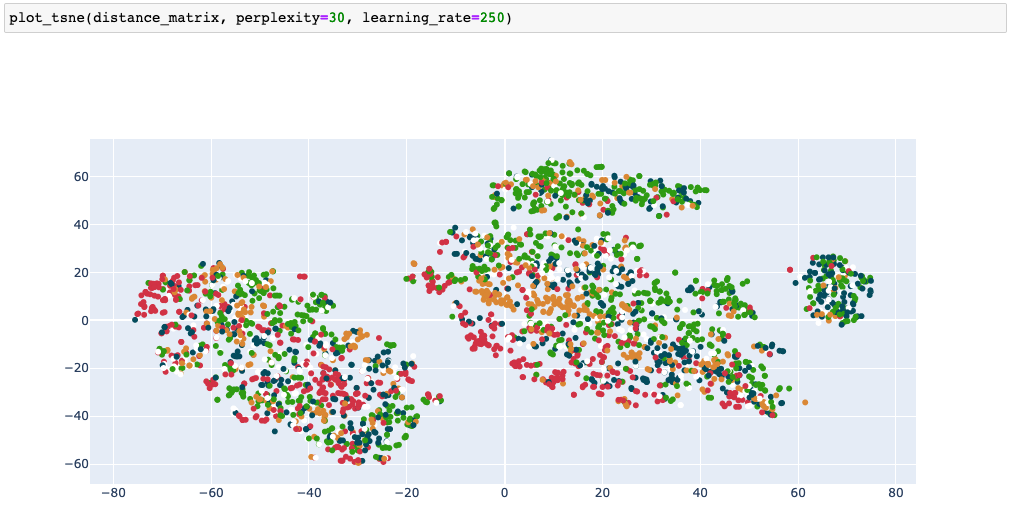
\includegraphics[width=\textwidth]{screenshots/pt_word_movers_distance_tsne1.png}
    \caption{Distance Matrix of the Word Mover's Distance with a pre-trained model (plotted with t-SNE)}
    \label{fig:wmd-pretrained-1}
  \end{center}
\end{figure}

\subsection{Conclusion}

\begin{itemize}
\item approaches work better on larger data sets, our data set was way to small
\item soft labeling was done by users
\item cannot be trusted, would have to be checked manually
\item the quality of the labels are bad - matching not as expected
\item common understanding of the domains was not available for the crowd workers, so domains may have been perceived differently
\item In the end, there would still be manual work involved to derive meaningful information with regard to what features or feature categories are wanted the most
\item finally, we can say that crowd re works to some extent: one can gather requirements, but it is very difficult to analyze them automatically or work with them any further 
\end{itemize}

% section analysis (end)
\section{Discussion}
\label{sec:discussion}
As expected, our dataset was probably too small to achieve any better results. In this context, it is important to know how the accuracy of the word2vec phrase detection dropped to 66\% when Mikolov et al. trained their model on a "smaller" dataset of 6 billion words\cite[p7]{mikolov_distributed_2013}. \emph{Smaller} at least in comparison to their final training set, but this is still a lot larger than our dataset by a factor of almost 120.000.

Also, all our word2vec approaches required to post-process the results using PCA. Though the PCA is a technique which is known for how well it can preserve the original information, some of the information will inevitably get lost. Our results may therefore have been impacted by the dimensionality reduction.

More time would have been needed for the evaluation of our results. Both the tags, as well as the application domains were set by the crowd-workers themselves. The quality of these assignemnts has not been proven yet and we used this data only for lack of proper testing data. For example, one of the requirements with the content "I want my smart home to sync with my biorhythm app and turn on some music that might suit my mood when I arrive home from work so that I can be relaxed" was related to the emph{Entertainment} domain. In our last approach this sentence was found to be in the \emph{Health} domain using the Word Mover's Distance. We could not say that this assignement was definitely wrong, though. So it could be we find our approach a lot more successful after a thorough analysis of all the clusters.

Finally, we lacked prior knowledge of the field of topic modeling and machine learning in general. Though we performed our research with technical and professional care in all conscience and under consideration of commonly accepted principles, there may be a lot of potential for further optimization (which goes beyond changing the hyper-parameters of our models).
%-

\section*{Acronyms}

\begin{tabbing}
spacespacespace \= space \kill
BOW \> Bag-of-Words\\
CBOW \> Continuous bag-of-words \\
CSV \> Comma Separated Value \\
LDA	\>	Latent Dirichlet allocation \\
ML \> Machine Learning\\
PCA \> Principal Component Analysis\\
RE	\>	Requirements Engineering \\
TF-IDF \> Term Frequency, Inverse Document Frequency \\
WMD \> Word Mover's Distance\\
\end{tabbing}

\bibliographystyle{splncs03}
\bibliography{references}

\end{document}